% Source: graduate-coursework/Sp26/CSCE763/Course_Assignments/HW3/HW3_CSCE_763_solutions.tex

\documentclass[border=4pt]{standalone}
\usepackage{amsmath}
\usepackage{amssymb}
\usepackage{graphicx}
\usepackage{tikz}
\usepackage{xcolor}
\usetikzlibrary{shapes.geometric, arrows.meta, positioning, patterns, calc}

\definecolor{USC_Garnet}{HTML}{73000A}
\definecolor{USC_Sandstorm}{HTML}{FFF2E3}
\definecolor{USC_Black90}{HTML}{363636}
\definecolor{USC_Black70}{HTML}{5C5C5C}
\definecolor{USC_Black50}{HTML}{A2A2A2}
\definecolor{USC_Black10}{HTML}{ECECEC}
\definecolor{USC_Honeycomb}{HTML}{65780B}
\definecolor{USC_Atlantic}{HTML}{466A9F}
\definecolor{USC_Congaree}{HTML}{1F414D}
\definecolor{USC_Rose}{HTML}{CC2E40}
\definecolor{USC_Grass}{HTML}{CED318}
\definecolor{USC_Horseshoe}{HTML}{65780B}
\definecolor{outputbg}{RGB}{245,245,245}

\begin{document}
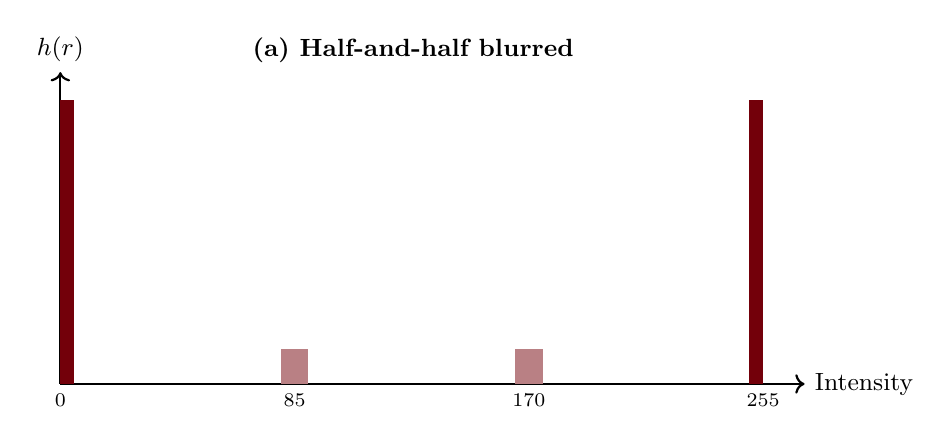
\begin{tikzpicture}[xscale=0.035, yscale=1.8]
% --- Histogram (a): Half-and-half blurred ---
\begin{scope}[shift={(0,0)}]
\draw[->, thick] (0,0) -- (270,0) node[right, font=\small] {Intensity};
\draw[->, thick] (0,0) -- (0,2.2) node[above, font=\small] {$h(r)$};
\node[above, font=\small\bfseries] at (128,2.2) {(a) Half-and-half blurred};
% Large spikes at 0 and 255
\fill[USC_Garnet] (0,0) rectangle (5,2.0);
\fill[USC_Garnet] (250,0) rectangle (255,2.0);
% Small intermediate values near 85 and 170
\fill[USC_Garnet!50] (80,0) rectangle (90,0.25);
\fill[USC_Garnet!50] (165,0) rectangle (175,0.25);
% Tick marks
\node[below, font=\scriptsize] at (0,0) {0};
\node[below, font=\scriptsize] at (85,0) {85};
\node[below, font=\scriptsize] at (170,0) {170};
\node[below, font=\scriptsize] at (255,0) {255};
\end{scope}
\end{tikzpicture}
\end{document}
